\section{Primera clase, 14 de agosto}

\subsection{Contenido de la materia}

\begin{itemize}
    \item Recorremos diferentes \textit{paradigmas} del mundo de la programación
    \item Las diferentes formas de trabajar abren la cabeza
    \item Conocer paradigmas acelera aprender lenguajes de programación
    \item Hay que acostumbrarse a leer \textit{papers}
\end{itemize}

\subsection{Modalidad de evaluación}

\begin{itemize}
    \item Hay trabajos prácticos
    \item Uno individual y uno grupal por cada mitad
    \item En total 4
\end{itemize}

\subsection{Lenguaje}

\begin{itemize}
    \item Forma de dar instrucciones a la máquina
    \item No darle mucha bola al marketing
    \item No nos vamos a concentrar tanto en lenguajes al principio
\end{itemize}

\subsection{Paradigmas}

\begin{itemize}
    \item Son \textit{formas de hacer las cosas}
    \item La programación se hace para humanos por humanos
    \item Aparecen y desaparecen ideas 
    \(\to\) aparecen y desaparecen paradigmas
    \item Primero se programaban físicamente
    \begin{itemize}
        \item Después Assembler 
        \item Lenguajes de alto nivel, el primero Fortran
    \end{itemize}
    \item En general, el mercado demanda orientación a objetos.
    \item El paradigma funcional es un poco extraño 
    \(\to\) puede servir computación cuántica
    \(\to\) Aunque todavía está por verse
    \item Conceptos que tenemos que manejar
    \begin{itemize}
        \item Declaratividad
        \item Transparencia 
        \item Abstracción 
        \item Asignación y unificación 
        \item Recursividad 
        \item Polimorfismo
    \end{itemize}
\end{itemize}

\begin{figure}[H]
    \centering
    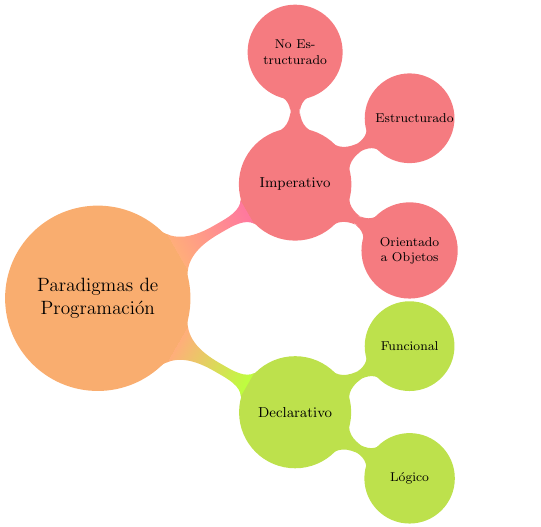
\includegraphics[width=.7\textwidth]{img/paradigmas.png}
\end{figure}

\subsection{Estructuras}
\begin{itemize}
    \item Bucle \textit{while}
    \item Condición \textit{if}
\end{itemize}

\subsection{Máquina de Turing}
\begin{itemize}
    \item Es lo mismo que los tres elementos de la estructura 
    \item En el \textit{paper} se demuestra
    \item Se computa todo lo computable
    \item El nivel de abstracción permite prescindir de estructuras como el \textit{goto}
\end{itemize}

\subsection{Online GDB}
\begin{itemize}
    \item Editor de texto y compilador online
    \item Tiene sus limitaciones pero sirve para cosas sencillas
    \item \url{https://www.onlinegdb.com/online_fortran_compiler}
\end{itemize}

\subsection{Limite del paradigma imperativo}
\begin{itemize}
    \item Como es secuencial, se complica la paralelización 
    \item Porque hay que hacerlo a mano 
    \item Los paradigmas declarativos se llevan mejor con este problema
    \item Programación funcional no tiene bucles: usa recursividad
\end{itemize}

\subsection{Temas de performance}
\begin{itemize}
    \item Puede o no ser relevante: 
    depende del balance entre velocidad de despliegue y costo de infraestructura
\end{itemize}

\subsection{Tarea}
\begin{itemize}
    \item Leer los textos de programación imperativa, los paradigmas
    \item \textit{Papers} opcionales
    \item Clase que viene: objetos, fundamentos POO 
\end{itemize}
